\documentclass{article}
\usepackage{graphicx}
\usepackage{hyperref}

\usepackage{enumitem}

\begin{document}

\title{Monte Carlo, Exercise Session 4}
\author{Alexey Sofiev, 013573003}
\date{}

\maketitle

%\begin{abstract}
%The abstract text goes here.
%\end{abstract}

\section{Exercise 1}
Files: Ex1.*. 

\textbf{Answer:} Figure \ref{fig:ex1_answer}.

\begin{figure}[!hbt]
	\centering
	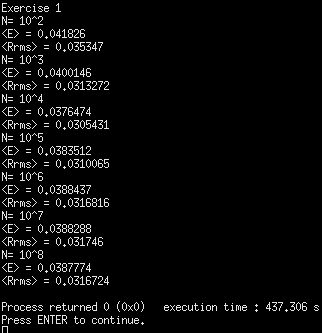
\includegraphics[width=4.3in]{ex1_answer}
	\caption{Ex1 answer.}
	\label{fig:ex1_answer}
\end{figure}

The other main question is log- plot, visualized in Figure \ref{fig:ex1_log}.

\begin{figure}[!hbt]
	\centering
	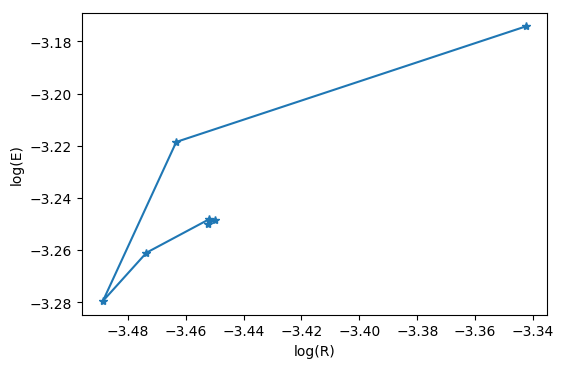
\includegraphics[width=4.3in]{ex1_log}
	\caption{Ex1 log plot.}
	\label{fig:ex1_log}
\end{figure}

And point in the upper right corner is obtained at the smallest N=100. (line connects to N=$10^3 \rightarrow 10^4 ...$) Therefore, the maximal absolute value of log(E) allowed should be 3.29.
\\
\\
\textbf{Solution details:}

%\begin{enumerate}[noitemsep]
	\textbf{1.} Algorithm is done basing on page 8 from \href{$https://moodle.helsinki.fi/pluginfile.php/714567/mod_resource/content/8/Markov_chain.pdf$}{Lecture notes on MCMC.}
%\end{enumerate}

	\textbf{2.} V is set to 1.
	
	\textbf{3.} Setting the range and $\triangle X_{max}$	

First let's take a look at the function without zooming. Figure \ref{fig:ex1_fig05}
\begin{figure}[!hbt]
	\centering
	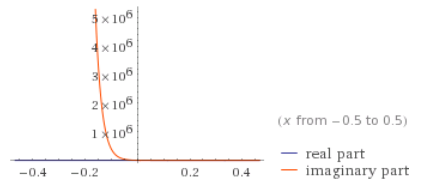
\includegraphics[width=4.3in]{ex1_fig05}
	\caption{Ex1, view on the function with 0.5. Function plotted with wolframalpha.}
	\label{fig:ex1_fig05}
\end{figure}

It can be noticed, that it is pretty flat, so now lets zoom into interesting part, Figure \ref{fig:ex1_fig008}.

\begin{figure}[!hbt]
	\centering
	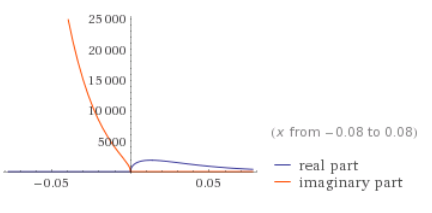
\includegraphics[width=4.3in]{ex1_fig008}
	\caption{Ex1, autozoom into real part. Function plotted with wolframalpha.}
	\label{fig:ex1_fig008}
\end{figure}

From Figure \ref{fig:ex1_fig008} it can be seen that setting $x_0$ to vary from 0 to 0.1, and $\triangle X_{max}$ to 0.05 is enough to generate most values. From lecture notes, it is told that $x_0$ doesn't really matter, on a long run, all the generated values will be distribution based distributed.

After generating random values and plotting them, the distribution obtained is presented in Figure \ref{fig:ex1_myDistribution}.

\begin{figure}[!hbt]
	\centering
	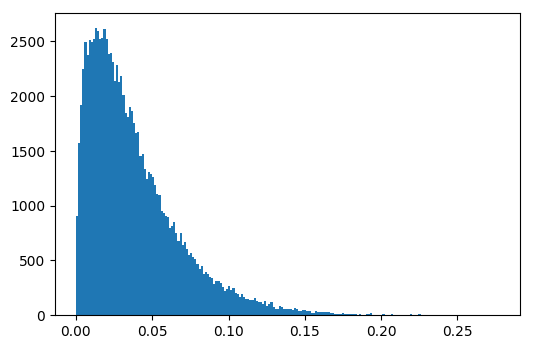
\includegraphics[width=4.3in]{ex1_myDistribution}
	\caption{Ex1, histogram of random values provided by the code.}
	\label{fig:ex1_myDistribution}
\end{figure}

The shape looks pretty much according to the theory presented in earlier figures.


\clearpage

\section{Exercise 2}
This exercise requires a lot of plotting, so will be done in Python using the Mersenne twister. File: Ex2.py
Images are automatically generated into a subdirectory data, and some of them are duplicated into tex folder.

\subsection*{Part 1, Given distribution:}

Using the lecture notes, the synthetic data, two of which are visualized in Figures \ref{fig:ex2_synt1} and \ref{fig:ex2_synt2}, is generated.
\begin{figure}[!hbt]
	\centering
	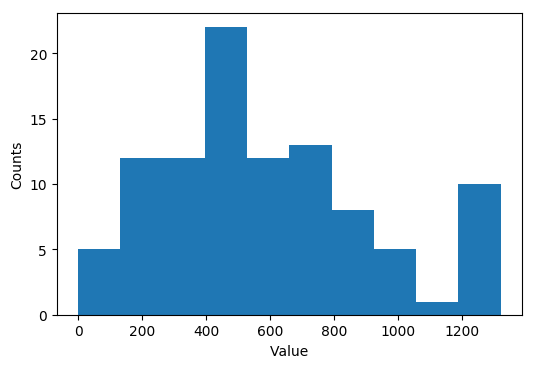
\includegraphics[width=4.3in]{ex2_synt1}
	\caption{Ex2, an example of generated synthetic data.}
	\label{fig:ex2_synt1}
\end{figure}

\begin{figure}[!hbt]
	\centering
	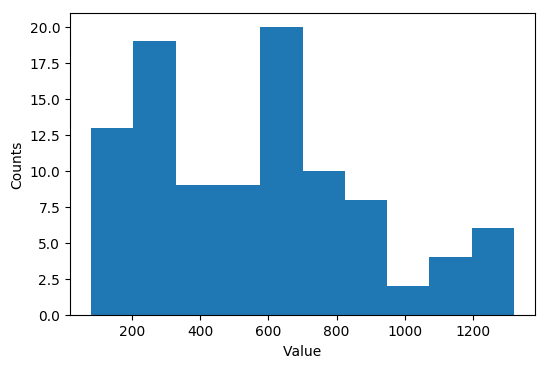
\includegraphics[width=4.3in]{ex2_synt2}
	\caption{Ex2, an example of generated synthetic data.}
	\label{fig:ex2_synt2}
\end{figure}

The generated synthetic data of 100, is has some sort of similarity, but they are still different.


For an example data lets calculate the CDF, and get 1 $\sigma$ uncertainty limit. Figure \ref{fig:ex2_cdf}.

\begin{figure}[!hbt]
	\centering
	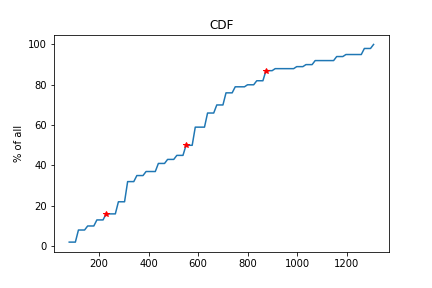
\includegraphics[width=4.3in]{ex2_cdf}
	\caption{Ex2, cdf of a single set with red starts marking 1$\sigma$ limits. x-axis is the data values.}
	\label{fig:ex2_cdf}
\end{figure}

The values of the edges are presented in Figure \ref{fig:ex2_singlecdfresult}. It can be noticed that they are not symmetric and variance is large.

\begin{figure}[!hbt]
	\centering
	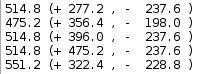
\includegraphics[width=4.3in]{ex2_singlecdfresult}
	\caption{Ex2, single measurements cdf 1$\sigma$ limits.}
	\label{fig:ex2_singlecdfresult}
\end{figure}

Now lets do the same to Poisson distribution.

\clearpage
\subsection*{Part 2, Poisson}
For generating Poisson random numbers the library provided function \textit{numpy.random.poisson(3)} will be used.

Few views on the generated datasets, Figures \ref{fig:ex2_poisson_synt0} and \ref{fig:ex2_poisson_synt3}.

\begin{figure}[!hbt]
	\centering
	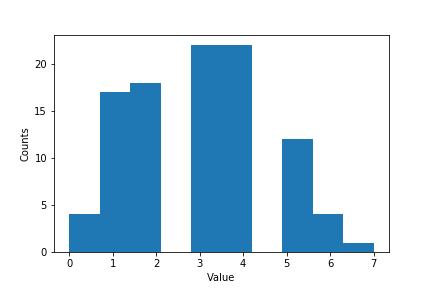
\includegraphics[width=4.3in]{ex2_poisson_synt0}
	\caption{Ex2, an example of Poisson-based generated data.}
	\label{fig:ex2_poisson_synt0}
\end{figure}

\begin{figure}[!hbt]
	\centering
	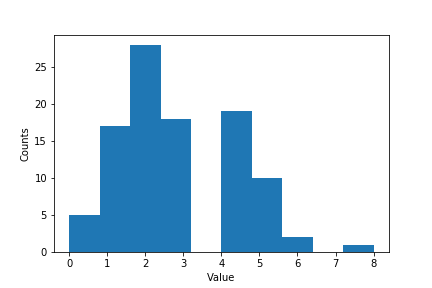
\includegraphics[width=4.3in]{ex2_poisson_synt3}
	\caption{Ex2, an example of Poisson-based generated data.}
	\label{fig:ex2_poisson_synt3}
\end{figure}

Some variations also occure because of small datasample, but the datasets are reminding the original distribution.


Next step is to create a CDF for the data, and get $1 \sigma$ limits.
\begin{figure}[!hbt]
	\centering
	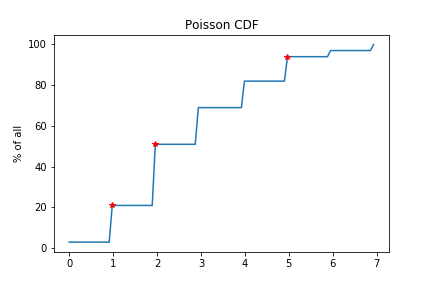
\includegraphics[width=4.3in]{ex2_poisson_cdf}
	\caption{Ex2, Poisson based CDF with 1$\sigma$ limits.}
	\label{fig:ex2_poisson_cdf}
\end{figure}

The limits are presented in Figure \ref{fig:ex2_poisson_singlecdfresult}

\begin{figure}[!hbt]
	\centering
	\includegraphics[width=4.3in]{ex2_poisson_singlecdfresult}
	\caption{Ex2, Poisson, CDF 1$\sigma$ limits.}
	\label{fig:ex2_poisson_singlecdfresult}
\end{figure}


\clearpage
\subsection*{Part 3, Summary}
In both cases 100 count data are deviating enough to break the Gaussian lower and upper bound symmetry. However in Poisson the middle point is more stable, in distr1.dat case, it varies more.


\end{document}